\documentclass[10pt,a4paper]{article}

\usepackage[a4paper,margin=1.6cm]{geometry}
\usepackage{graphicx}
\usepackage{amsmath}
\usepackage{booktabs}
\usepackage{float}
\usepackage{wrapfig}
\usepackage{xcolor}
\usepackage{listings}
\usepackage{hyperref}

\setlength{\parindent}{0pt}
\setlength{\parskip}{3pt}
\hypersetup{colorlinks=true,urlcolor=blue}

\lstset{
    language=Python,
    basicstyle=\ttfamily\scriptsize,
    breaklines=true,
    frame=single,
    numbers=none,
    showstringspaces=false
}

\begin{document}

\begin{center}
    {\Large\textbf{EN3160 -- Assignment 02}}\\[3pt]
    Name: Saruka U. \hfill Index No: 230585C\\
    GitHub: \url{https://github.com/Saruka03/EN3160-Assignment-02}
\end{center}

\vspace{-4pt}
\hrule
\vspace{5pt}

% ============================================================
\section*{1. Blob Detection in the Sunflower Image}

\begin{wrapfigure}{r}{0.40\textwidth}
   % \centering
    \vspace{-10pt}
    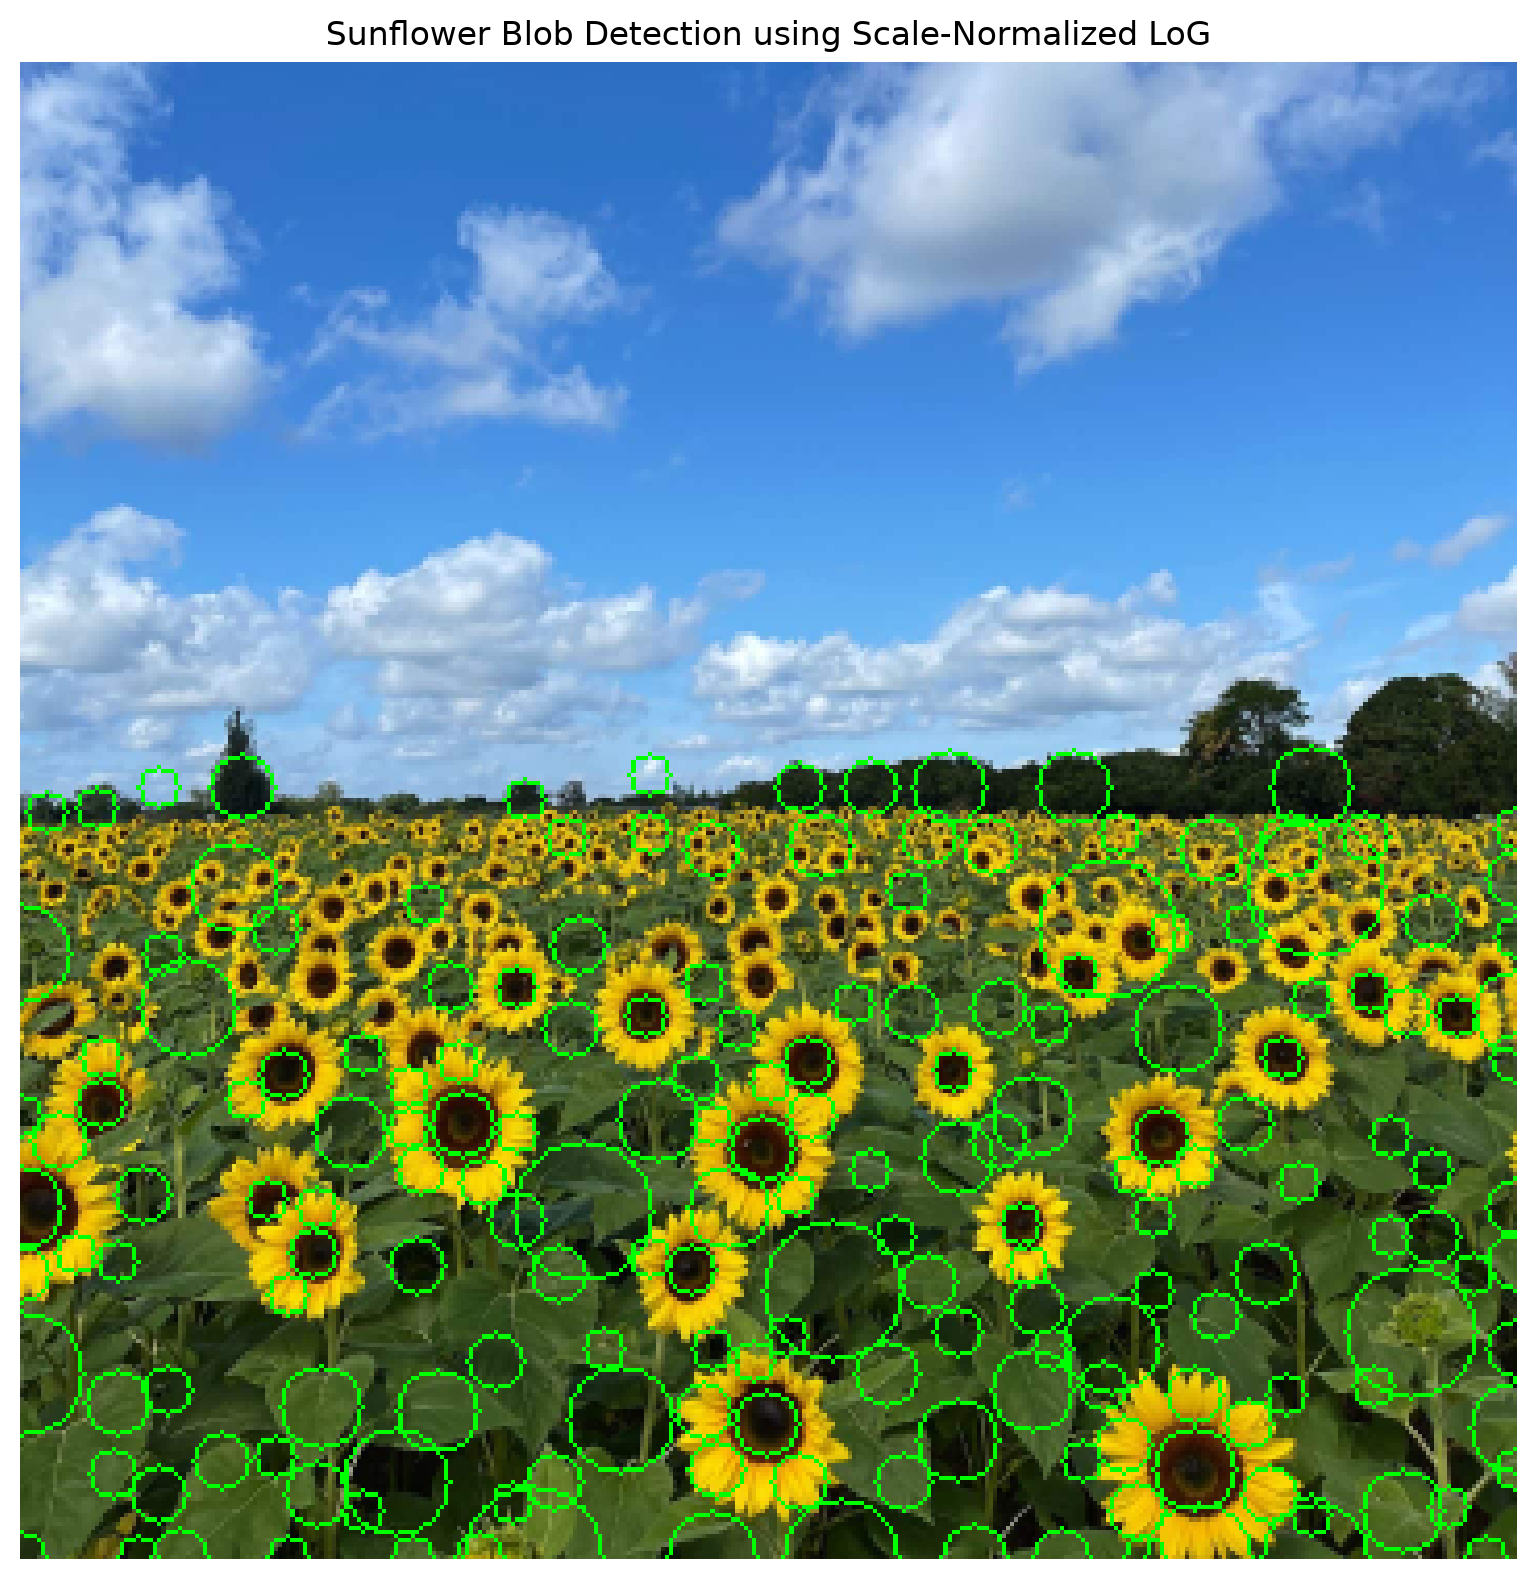
\includegraphics[width=0.38\textwidth]
    {../outputs/q1_sunflowers_plot.png}
    \caption{Detected blobs in the sunflower image.}
    \label{fig:q1-detections}
    \vspace{-10pt}
\end{wrapfigure}

The sunflower image was processed using a scale-normalized
Laplacian of Gaussian (LoG) detector. The scale-space was
evaluated over 20 scales in the range
$\sigma=2.2$ to $\sigma=12.0$. Local maxima were selected
using a response threshold of 12\% of the maximum response.
Detections with $\sigma<2.9$ were excluded, and spatial
suppression with a 10-pixel centre distance was applied.

The final experiment retained 185 blob detections. These
include sunflower heads as well as some background structures;
therefore, the number of detections is not an exact sunflower
count.


The five largest detected circles, ranked by radius, are
listed in Table~\ref{tab:largest-circles}. The approximate
radius was calculated using $r=\sqrt{2}\sigma$.

\begin{table}[H]
    \small
    %\caption{Five largest detected circles.}
    \label{tab:largest-circles}
    \begin{tabular}{ccccc}
        \toprule
        Centre $(x,y)$ & Radius (pixels) & $\sigma$ & Response\\
        \midrule
        $(311,198)$ & 16.97056 & 12.00000 & 0.10385\\
        $(123,359)$ & 16.97056 & 12.00000 & 0.12126\\
        $(195,295)$ & 16.97056 & 12.00000 & 0.12687\\
        $(261,208)$ & 16.97056 & 12.00000 & 0.10860\\
        $(135,276)$ & 16.97056 & 12.00000 & 0.08139\\
        \bottomrule
    \end{tabular}
\end{table}


The detector retained 185 blobs over 20 scales in the range
$\sigma=2.2$ to $\sigma=12.0$. The largest detected radius
was 16.97 pixels at $\sigma=12.0$. Since the largest
detections occur at the maximum tested scale, some circles
may represent larger image structures rather than individual
sunflowers.

\vspace{4pt}
% ============================================================
\section*{2. RANSAC Line and Circle Fitting}

\begin{wrapfigure}{r}{0.48\textwidth}
    
    \vspace{-10pt}
    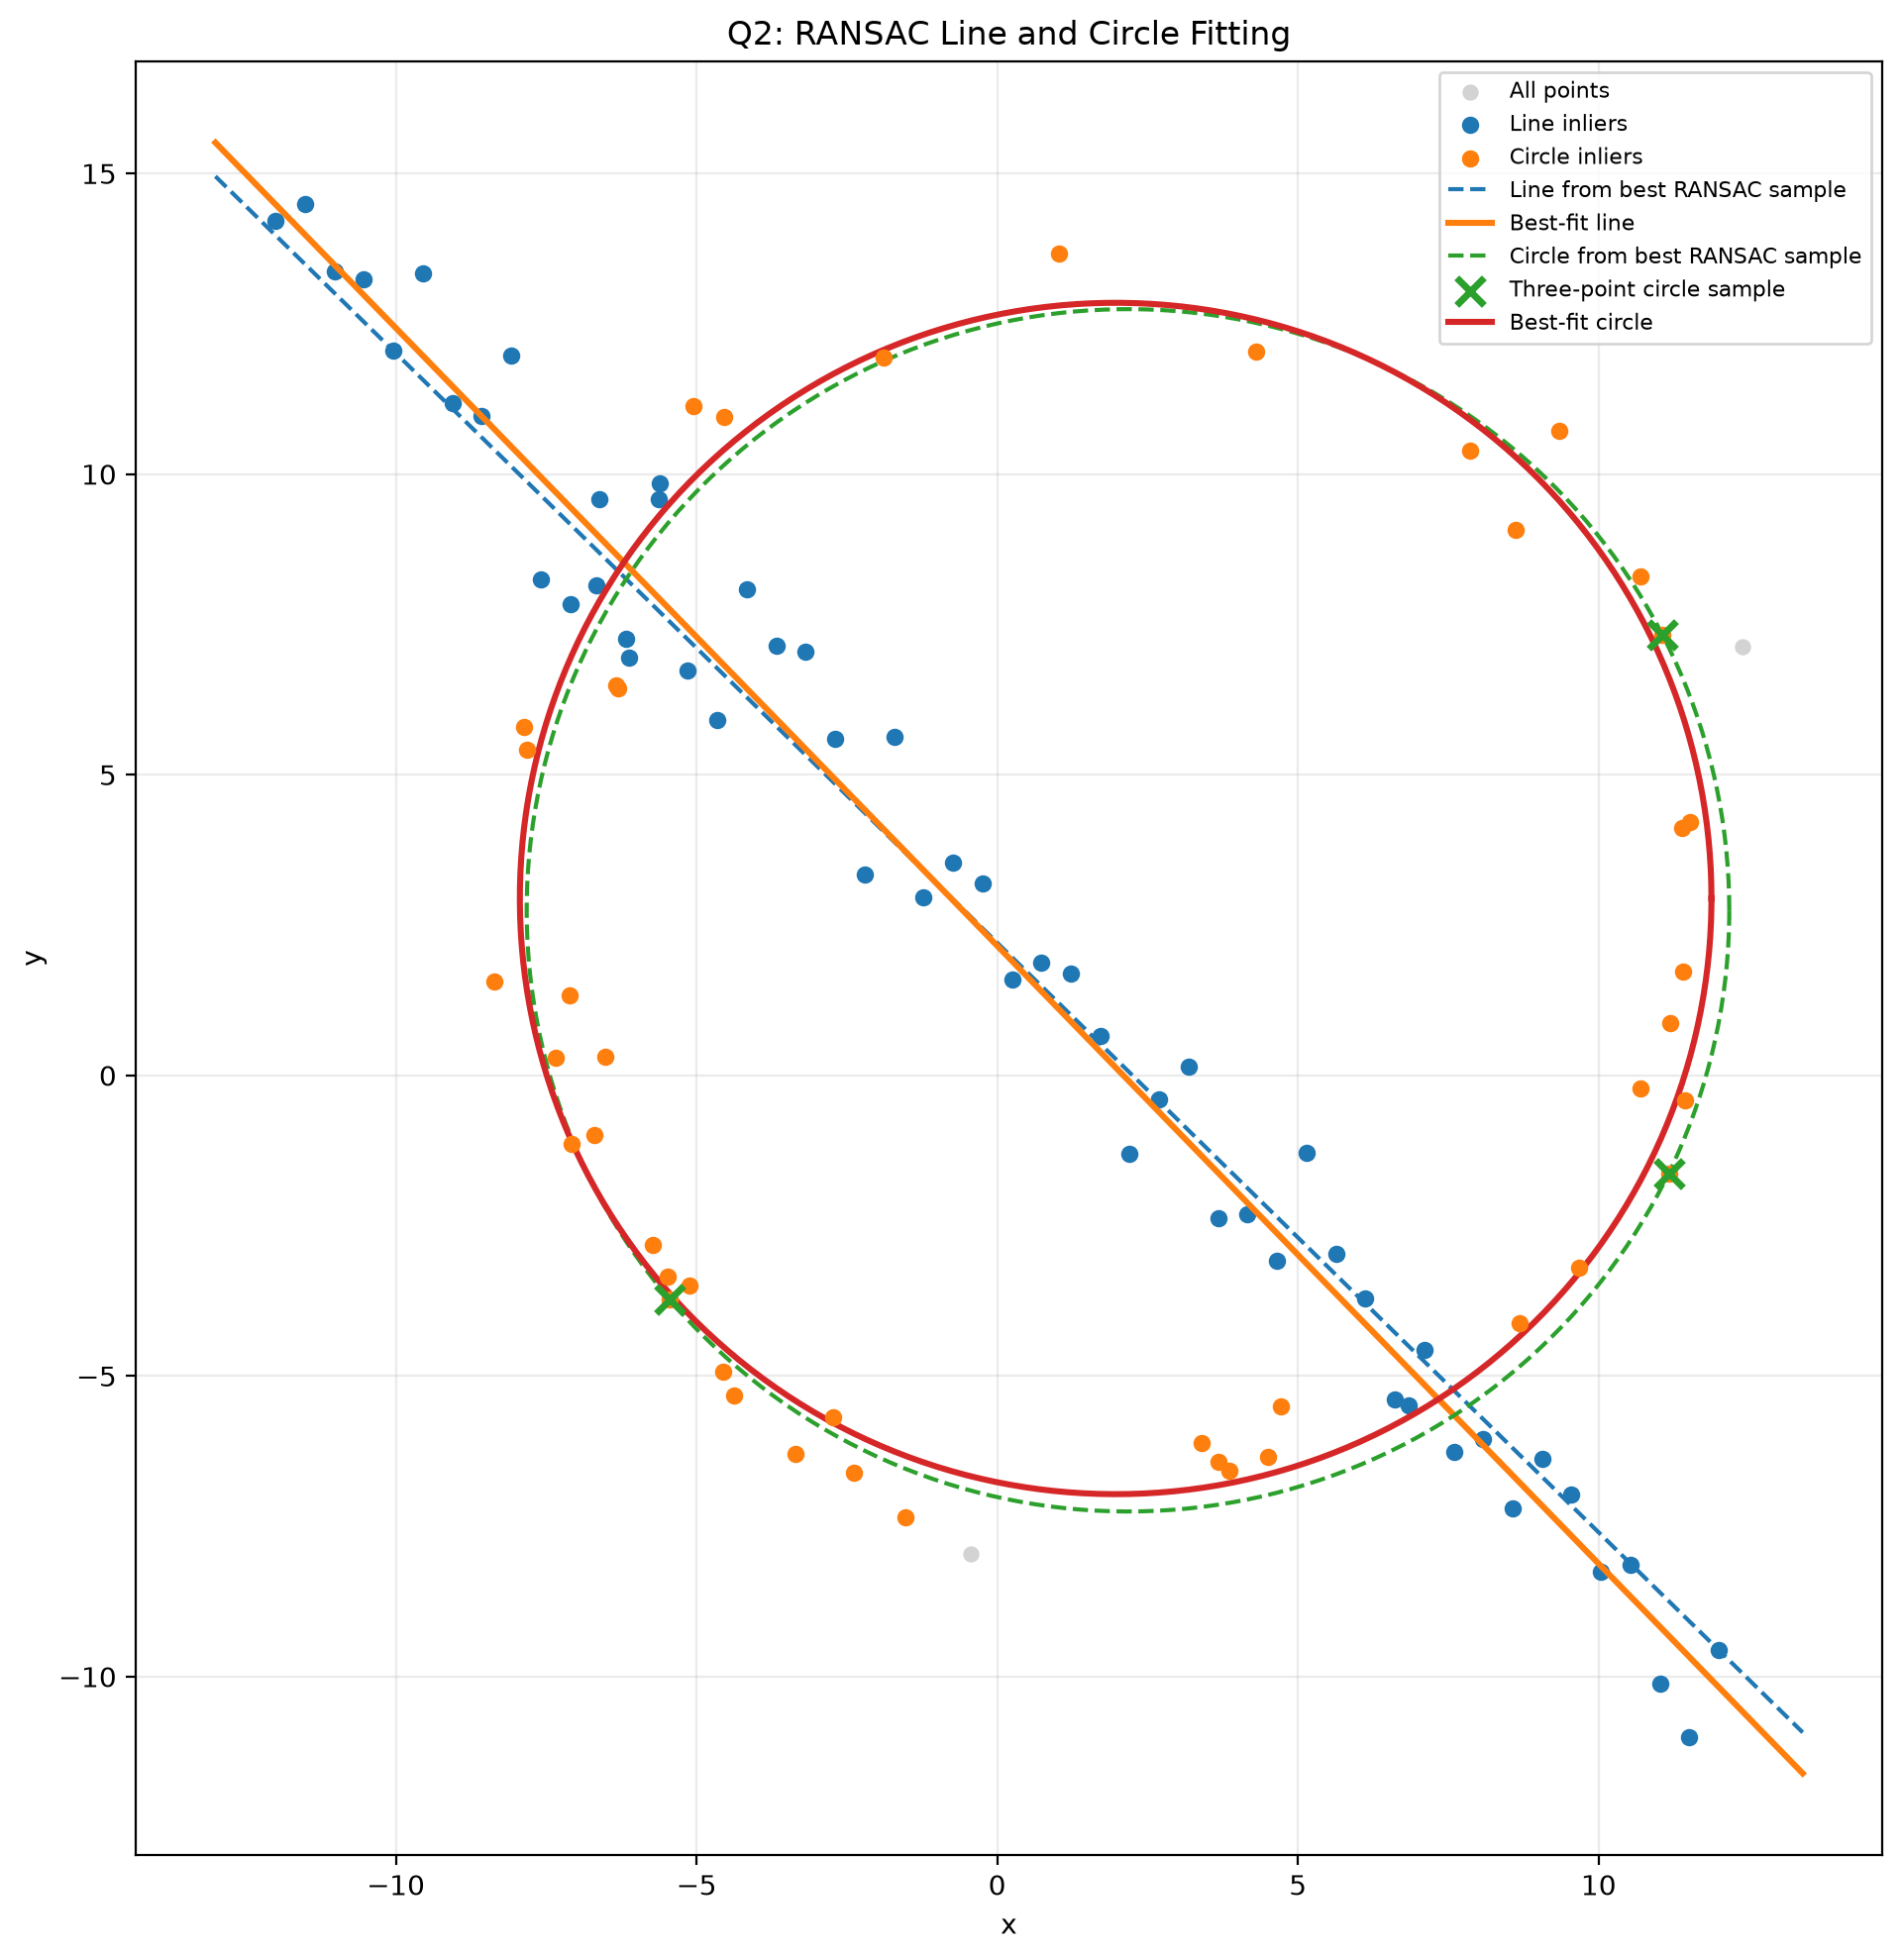
\includegraphics[width=0.46\textwidth]
    {../outputs/q2_ransac_line_circle.png}
    %\caption{RANSAC line and circle fitting.}
    \label{fig:q2-ransac}
    \vspace{-10pt}
\end{wrapfigure}

RANSAC was implemented to estimate a line first, followed
by a circle fitted to the points remaining after removing
the line inliers. The line inlier threshold was 1.4, and
the circle radial-error threshold was 1.2.

The estimated line parameters were
\[
a=0.716670,\quad b=0.697413,\quad d=1.502897.
\]
Therefore, the fitted line is
\[
0.716670x+0.697413y=1.502897.
\]
The unit-normal constraint was satisfied:
$\sqrt{a^2+b^2}=1.000000$. The final line contained
54 inliers out of 100 points.

The estimated circle centre and radius were
\[
(c_x,c_y)=(1.969390,\;2.942512),\qquad r=9.907175.
\]
The circle contained 44 inliers. These estimates are close
to the ground-truth centre $(2,3)$ and radius $10$.

The plot shows the best sample models, the refined models,
and the detected inlier sets. Some points may be assigned
to the wrong model because of noise and spatial overlap.

\subsection*{What if the circle were fitted first?}

RANSAC could first sample three points to estimate candidate
circles and select the model with the largest radial-error
consensus. After removing the circle inliers, line fitting
could be performed on the remaining points. This reversed
order can also work, although the result depends on sampling,
noise, and the chosen thresholds.

\subsection*{Important implementation details}

The line RANSAC loop samples two points and counts inliers
using perpendicular distance. The circle RANSAC loop samples
three points and counts inliers using radial error. The best
models are refined using total least squares for the line and
squared radial-error minimization for the circle.

\begin{lstlisting}
# Line inlier test
line_error = np.abs(X @ np.array([a, b]) - d)
line_inliers = line_error < 1.4

# Circle inlier test
radial_error = np.abs(
    np.linalg.norm(points - center, axis=1) - radius
)
circle_inliers = radial_error < 1.2
\end{lstlisting}

\end{document}